\input{preamble}
\begin{document}

\title{
Trabalho de Álgebra Linear Computacional \hspace{2.0ex} 26.1\\
\textit{Pitch Shifting} em Tempo Real com STFT e \textit{Phase Vocoder}
}

\author{
    Tiago Maia de Lacerda Brasil\inst{1}
}

\address{
    %---------------------------------------------------------------
    Instituto de Computação -- Universidade Federal Fluminense (UFF)\\
    Niterói -- RJ -- Brasil -- 24210-346
    \email{tiagomlbrasil@gmail.com}
    %---------------------------------------------------------------
}
\maketitle

\begin{abstract}
    Este trabalho apresenta o desenvolvimento de um plugin de \textit{pitch shifting} em tempo real baseado na Transformada de Fourier de Curta Duração (STFT) e em técnicas de phase vocoder. O algoritmo foi implementado em C++17 utilizando o framework JUCE no formato VST3.

    São discutidos os fundamentos teóricos relacionados à análise de sinais no domínio das frequências e as principais decisões de implementação adotadas no desenvolvimento do algoritmo, incluindo processamento por quadros, estimação de frequências instantâneas e reconstrução temporal do sinal.

    Por fim, são apresentadas algumas limitações práticas da abordagem utilizada e possíveis extensões baseadas em técnicas descritas na literatura.
\end{abstract}

\noindent\textit{\textbf{Keywords}}: processamento digital de sinais, STFT, \textit{phase vocoder}, \textit{pitch shifting}, áudio em tempo real

% Nosso objetivo final é construir um programa que altera o tom de um sinal de áudio. Queremos ser capazes de operar no espaço de frequencias, e para isso existe a transformada de Fourier. Mas ela espera um sinal periodico, e queremos operar em tempo real. Entao usamos curtas janelas de analálise. Mas isso gera artefatos nas bordas. Entao misturamos janelas consecutivas com uma função que amortece a transição entre as janelas <comentar sobre a necessidade de uma normalizacao, a ser calculada dependendo da funcao de windowing e pela forma como ocorre o overlap>. Otimo, conseguimos operar nas frequencias em tempo real, mas o som está horrível <Explicar spectral leakage e introduzir o conceito de phase vocoder>. Conseguimos transformar o sinal no espaço de frequencias e de volta no tempo sem grandes artefatos, mas ainda nao fizemos nada de pitch shifting. <Definir uma oitava, semitons e que podemos subir ou descer uma oitava de uma nota multiplicando sua frequencia por uma certa potencia de 2>. Entao, tendo em maos quantos semitons queremos shiftar, podemos calcular um novo espectro de frequencias onde cada banda de frequencia do sinal original está movida por um fator 2^(semitons/12) e interpolar nas k bins de frequencia suportadas pela nossa janela da fft, mas isso pode estar fora do limite representável pela nossa janela da FFT (shift up), ou ainda moverem todos para uma região muito pequena e causar um embaralhamento das frequencias (shift down).

%<Em momento oportuno, solidificar os conceitos de overlap-add, análise e síntese, ring buffers, e comentar a latencia inerente ao phase-vocoder, onde uma primeira janela precisa ser montada, atrasando o sinal pelo tamanho da janela>

\section{Introdução}\label{sec:intro}

O processamento digital de sinais de áudio está presente em diversas aplicações modernas, incluindo sistemas multimídia, ferramentas de produção musical e efeitos sonoros em tempo real. Nesse contexto, técnicas de análise no domínio das frequências permitem modificar diferentes características do sinal, como timbre, conteúdo harmônico e tom.

Entre essas aplicações, algoritmos de \textit{pitch shifting} permitem alterar o tom percebido de um sinal sem modificar significativamente sua duração temporal. Uma das abordagens mais utilizadas para esse tipo de processamento baseia-se na Transformada de Fourier de Curta Duração (STFT) e em técnicas de \textit{phase vocoder} \cite{dolson1986,flanagan1966}, que permitem analisar e modificar componentes do sinal no domínio das frequências.

Entretanto, a implementação desses algoritmos em tempo real envolve desafios relacionados à reconstrução temporal do sinal, à preservação de coerência entre fases e às limitações impostas pelo processamento baseado em quadros.

Este trabalho apresenta o desenvolvimento de um plugin de \textit{pitch shifting} em tempo real baseado em STFT e \textit{phase vocoder}. Inicialmente, são discutidos os fundamentos teóricos relacionados à STFT e ao \textit{phase vocoder}. Em seguida, são descritas as decisões de implementação adotadas no desenvolvimento do algoritmo e suas principais limitações práticas.




\section{Fundamentação teórica}\label{sec:fundamentacao}

\subsection{Representação Espectral de Sinais}

Sinais de áudio são tradicionalmente representados no domínio do tempo, onde cada amostra descreve a amplitude do sinal em um determinado instante. Essa representação é adequada para captura, armazenamento e reprodução do áudio, mas nem sempre é a forma mais conveniente para analisar determinadas características do sinal ou realizar modificações específicas.

Uma representação alternativa consiste em descrever o sinal no domínio das frequências. Nesse contexto, o sinal passa a ser interpretado como uma combinação de diversas componentes senoidais com diferentes amplitudes, frequências e fases \cite{oppenheim1999}. Essa abordagem permite identificar de maneira mais direta o conteúdo espectral presente no áudio e facilita operações relacionadas à manipulação de frequências.

Diversas técnicas de processamento digital de sinais utilizam representações espectrais para realizar tarefas como filtragem, remoção de ruído, análise de conteúdo harmônico e alteração de características como tom e timbre. No caso deste trabalho, a representação no domínio das frequências é particularmente relevante por permitir a implementação de algoritmos de \textit{pitch shifting}, nos quais as componentes espectrais do sinal são deslocadas de forma controlada para produzir alterações no tom percebido do som.

\subsection{Transformada Discreta de Fourier}

A representação espectral de um sinal discreto pode ser obtida por meio da Transformada Discreta de Fourier (DFT, do inglês \textit{Discrete Fourier Transform}). Essa transformação converte um conjunto finito de amostras no domínio do tempo em uma representação equivalente no domínio das frequências, permitindo identificar quais componentes senoidais contribuem para a formação do sinal analisado.

Matematicamente, a DFT de uma sequência discreta \(x[n]\) de comprimento \(N\) é definida por

\begin{equation}
X[k] = \sum_{n=0}^{N-1} x[n] e^{-j\frac{2\pi}{N}kn},
\end{equation}

onde \(X[k]\) representa o coeficiente espectral associado ao índice \(k\). Cada coeficiente complexo contém informações sobre a magnitude e a fase de uma determinada componente de frequência presente no sinal.

A resolução espectral obtida pela DFT depende do número de amostras analisadas. Para uma frequência de amostragem \(f_s\), os coeficientes espectrais correspondem a frequências igualmente espaçadas por

\begin{equation}
\Delta f = \frac{f_s}{N}.
\end{equation}

Essas posições discretas no espectro são frequentemente denominadas \textit{bins}. Cada \textit{bin} representa uma faixa de frequências centrada em um valor específico, permitindo descrever o conteúdo espectral do sinal de forma discreta.

Embora a DFT forneça uma representação completa do conteúdo espectral de um conjunto de amostras, seu custo computacional cresce quadraticamente com o tamanho do sinal. Em aplicações de processamento de áudio em tempo real, esse custo pode se tornar proibitivo, motivando o uso de algoritmos mais eficientes para seu cálculo.

\subsection{Transformada Rápida de Fourier}

A Transformada Rápida de Fourier (FFT, do inglês \textit{Fast Fourier Transform}) consiste em uma família de algoritmos capazes de calcular a DFT de forma mais eficiente. Diferentemente da DFT, que requer um número de operações proporcional a \(N^2\), algoritmos FFT reduzem essa complexidade para \(N \log_2 N\), tornando viável a análise espectral de sinais extensos e aplicações de processamento em tempo real.

A redução do custo computacional é obtida pela exploração de simetrias e redundâncias presentes nos coeficientes da DFT. Em particular, algoritmos do tipo Cooley-Tukey dividem recursivamente o problema original em transformadas menores, combinando posteriormente os resultados para obter o espectro completo do sinal.

Embora a FFT produza exatamente os mesmos coeficientes espectrais que a DFT, sua eficiência computacional tornou seu uso praticamente universal em aplicações de processamento digital de sinais. No contexto deste trabalho, a FFT é empregada tanto na etapa de análise espectral quanto na reconstrução do sinal por meio da transformada inversa.

\subsection{Transformada de Fourier de Curta Duração}

A DFT fornece uma representação espectral de um conjunto finito de amostras. No entanto, ao analisar todas as amostras simultaneamente, perde-se a informação sobre em que instante cada componente espectral ocorre no sinal.

Além disso, em aplicações de áudio em tempo real não é possível aguardar a captura completa do sinal antes de realizar seu processamento. Torna-se necessário analisar e transformar pequenas porções do áudio à medida que novas amostras são recebidas.

A Transformada de Fourier de Curta Duração (STFT, do inglês \textit{Short-Time Fourier Transform}) baseia-se nesse princípio \cite{oppenheim1999}. O sinal é dividido em segmentos de curta duração, denominados quadros (\textit{frames}), e uma transformada é aplicada individualmente a cada um deles.

O resultado é uma sequência de espectros capaz de descrever a evolução temporal das frequências que compõem o sinal, estabelecendo uma representação simultânea nos domínios do tempo e da frequência.

\subsection{Reconstrução Temporal}

% TODO: Revisar a escrita desta seção

A segmentação de um sinal em quadros sucessivos permite realizar análises localizadas no tempo, mas introduz um novo desafio. Ao extrair um trecho finito de um sinal contínuo, criam-se descontinuidades artificiais nas extremidades do quadro analisado.

Essas descontinuidades podem introduzir componentes espectrais que não estavam presentes no sinal original, fenômeno conhecido como \textit{spectral leakage}. Como consequência, a energia associada a uma determinada frequência deixa de permanecer concentrada em uma única região do espectro e passa a se distribuir entre múltiplos \textit{bins}, dificultando a análise e o processamento do sinal.

Uma forma de reduzir esse efeito consiste em multiplicar cada quadro por uma função de janela antes da aplicação da transformada. Essa operação atenua gradualmente as amplitudes próximas às extremidades do segmento, reduzindo as descontinuidades introduzidas pelo recorte temporal.

Entretanto, o janelamento modifica a amplitude do sinal analisado, tornando inadequada a simples concatenação dos quadros reconstruídos. Para preservar a continuidade temporal e a amplitude original do sinal, os quadros sintetizados são parcialmente sobrepostos e posteriormente somados por meio da técnica de \textit{overlap-add} \cite{griffin1984}.

\subsection{Magnitude e Fase no Domínio Espectral}

Os coeficientes produzidos pela DFT são valores complexos que podem ser representados em termos de magnitude e fase. A magnitude está associada à intensidade de uma determinada componente espectral, enquanto a fase descreve sua posição relativa no tempo.

Em muitas aplicações, a magnitude fornece informações suficientes para caracterizar aspectos importantes do sinal, como a distribuição de energia entre diferentes frequências. Entretanto, a reconstrução do sinal original a partir de sua representação espectral depende tanto da magnitude quanto da fase de cada componente \cite{dolson1986}. Alterações arbitrárias nas fases espectrais podem modificar significativamente a forma de onda resultante, mesmo quando as magnitudes permanecem inalteradas. Em sinais de áudio, esse tipo de alteração pode resultar em transientes menos definidos e em artefatos perceptíveis, frequentemente descritas como sons metálicos, artificiais ou vazios \cite{laroche1999}.

% TODO: Revisar a descrição dos artefatos de áudio acima

Embora alterações inadequadas de fase possam produzir resultados indesejados, a fase constitui uma propriedade fundamental do sinal. Efeitos de áudio como \textit{phasers} e \textit{flangers} exploram deliberadamente relações de fase para produzir características sonoras específicas. Assim, o objetivo não é eliminar a informação de fase, mas preservá-la ou manipulá-la de forma controlada.

Na STFT, cada componente espectral é observada ao longo de uma sequência de quadros consecutivos. A variação de fase entre essas observações contém informações sobre a evolução temporal do sinal e permite estimar com maior precisão a frequência associada a cada componente espectral. Técnicas capazes de explorar essa informação durante os processos de análise e síntese são conhecidas como \textit{phase vocoders}.

\subsection{\textit{Phase vocoders}}

Cada \textit{bin} da STFT possui uma magnitude e uma fase associadas. Para uma senoide cuja frequência coincide exatamente com a frequência central de um \textit{bin}, a evolução da fase entre quadros consecutivos pode ser prevista a partir da frequência da senoide e do intervalo temporal entre análises.

Nesse caso, o avanço de fase esperado entre dois quadros consecutivos é dado por

\begin{equation}
\Delta\phi_{esp}
=
2\pi k \frac{H}{N},
\end{equation}

onde \(k\) representa o índice do \textit{bin}, \(H\) o passo entre análises (\textit{hop size}) e \(N\) o tamanho da transformada.

Entretanto, sinais reais raramente apresentam componentes perfeitamente alinhadas às frequências centrais da transformada. Além disso, efeitos como o \textit{spectral leakage} fazem com que a energia de uma componente seja distribuída entre múltiplos \textit{bins}. Como consequência, a variação de fase observada nem sempre corresponde ao avanço esperado para a frequência central do \textit{bin}.

A diferença entre o avanço de fase observado

\begin{equation}
\Delta\phi_{obs}
=
\phi_m - \phi_{m-1},
\end{equation}

e o avanço esperado contém informações sobre a frequência efetiva da componente analisada. A partir dessa diferença, é possível estimar uma frequência mais precisa do que aquela fornecida apenas pela posição do \textit{bin} na transformada. A frequência angular instantânea pode ser estimada \cite{dolson1986} por

\begin{equation}
\omega_{inst}
=
\frac{2\pi k}{N}
+
\frac{\Delta\phi_{obs}-\Delta\phi_{esp}}{H}.
\end{equation}

A análise da evolução temporal das fases, a estimação das frequências efetivas das componentes espectrais e a posterior reconstrução coerente do sinal constituem os princípios fundamentais do \textit{phase vocoder} \cite{flanagan1966,dolson1986}. Essa abordagem permite manipular componentes espectrais preservando relações temporais importantes do sinal, servindo como base para aplicações de \textit{time stretching} e \textit{pitch shifting}.

\subsection{\textit{Pitch shifting}}

Uma oitava corresponde ao intervalo entre duas notas cujas frequências diferem por um fator de dois. Dessa forma, uma nota com frequência \(f\) possui sua oitava superior em \(2f\) e sua oitava inferior em \(f/2\).

No sistema de doze temperamentos iguais, predominante na música contemporânea, a oitava é dividida em doze semitons igualmente espaçados. Nessa convenção, um deslocamento de \(s\) semitons corresponde à razão de frequências

\begin{equation}
r = 2^{s/12}.
\end{equation}

Assim, aumentar o tom percebido de um sinal em \(s\) semitons equivale a multiplicar suas frequências por \(2^{s/12}\), enquanto reduzi-la equivale à aplicação do mesmo fator para valores negativos de \(s\).

Uma vez obtida uma representação espectral composta por magnitudes e frequências estimadas pelo \textit{phase vocoder}, o processo de \textit{pitch shifting} consiste em reposicionar essas componentes espectrais segundo a razão desejada. Como as novas frequências raramente coincidem exatamente com as posições discretas dos \textit{bins} da transformada, torna-se necessário estimar sua contribuição para o espectro sintetizado por meio de técnicas de interpolação.

Dessa forma, a combinação entre a análise espectral fornecida pela STFT, a estimação de frequência realizada pelo \textit{phase vocoder} e o reposicionamento das componentes espectrais permite alterar o tom percebido de um sinal preservando sua duração temporal original.
\section{Metodologia}\label{sec:metodologia}

O algoritmo desenvolvido neste trabalho foi implementado em C++17 utilizando o framework JUCE, na forma de um plugin VST 3 (\textit{Virtual Studio Technology 3}) compatível com diferentes DAWs (do inglês, \textit{Digital Audio Workstation}).

\subsection{Modelo de Processamento em Tempo Real}

Nesse modelo de execução, o framework fornece periodicamente blocos de amostras do sinal de áudio e espera receber, ao final de cada chamada, um bloco de saída com a mesma quantidade de amostras processadas.

Como o tamanho desses blocos não necessariamente coincide com o tamanho dos quadros utilizados pela STFT, torna-se necessário utilizar estruturas intermediárias para armazenar as amostras do sinal antes e após o processamento espectral.

As amostras recebidas são continuamente escritas em um buffer circular de análise até que exista informação suficiente para compor um novo quadro da FFT. Após o processamento, os quadros reconstruídos são acumulados em um buffer circular de síntese por meio da técnica de \textit{overlap-add}, de onde o framework consome continuamente as amostras de saída.

\subsection{Análise Espectral por Quadros}

Sempre que o buffer de análise acumula amostras suficientes para compor um novo quadro, o algoritmo extrai uma janela de tamanho fixo para a realização da FFT.

O tamanho da transformada determina simultaneamente a resolução espectral da análise e a latência introduzida pelo algoritmo. Considerando uma taxa de amostragem \(f_s\), a maior frequência representável é dada pela frequência de Nyquist, correspondente a \(f_s/2\). Dessa forma, para um sinal amostrado a \(44{,}1\,\mathrm{kHz}\), o espectro analisado cobre frequências de até aproximadamente \(22\,\mathrm{kHz}\), abrangendo a faixa audível típica da audição humana.

Além disso, para uma FFT de tamanho \(N\), a resolução em frequência é dada por

\begin{equation}
\Delta f = \frac{f_s}{N},
\end{equation}

indicando o espaçamento entre \textit{bins} espectrais consecutivos. Quadros maiores fornecem maior precisão espectral, porém aumentam a latência e reduzem a resolução temporal do algoritmo.

Neste trabalho, utilizou-se uma FFT de tamanho \(4096\), valor escolhido como compromisso entre resolução espectral, custo computacional e latência perceptível durante o processamento em tempo real.

Antes da transformada, cada quadro é multiplicado por uma função de janela. Neste trabalho, utilizou-se uma janela raiz de Hann (\textit{sqrt Hann window}) em conjunto com uma taxa de sobreposição de 75\%, permitindo a reconstrução contínua do sinal por meio da técnica de \textit{overlap-add} \cite{griffin1984}.

% TODO: Adicionar imagem ilustrando a função de janelamento e múltiplos quadros sobrepostos no tempo

\begin{figure}[ht]
    \centering
    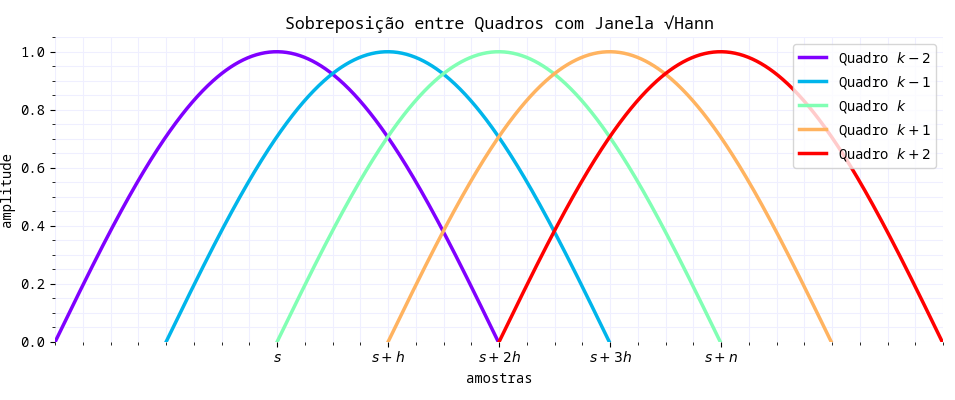
\includegraphics[width=\linewidth]{figures/overlap-add.png}
    \caption{Sobreposição entre quadros utilizando janela raiz de Hann e taxa de sobreposição de 75\%.}
    \label{fig:overlap-add}
\end{figure}

Como múltiplos quadros sobrepostos contribuem simultaneamente para uma mesma região temporal do sinal reconstruído, torna-se necessário aplicar um fator de normalização durante a síntese. Esse procedimento evita variações artificiais de amplitude causadas pela superposição das janelas.

\subsection{Estimação de Frequência pelo \textit{Phase Vocoder}}

Após a obtenção do espectro complexo de cada quadro, o algoritmo extrai a magnitude e a fase associadas a cada \textit{bin} espectral. As fases do quadro anterior são armazenadas para permitir a análise da evolução temporal de cada componente entre quadros consecutivos.

O avanço de fase esperado para cada \textit{bin} é calculado em função de sua frequência central, do tamanho da FFT e do intervalo entre análises. Em seguida, o algoritmo calcula a diferença entre as fases observadas em quadros consecutivos.

\begin{minted}{cpp}
float deltaPhase = phase - previousAnalysisPhases[k];

float expectedPhaseAdvance =
    tau * static_cast<float>(k)
    * static_cast<float>(analysisHopSamples)
    / static_cast<float>(frameSamples);
\end{minted}

Como fases são representadas modularmente no intervalo \([-\pi, \pi]\), diferenças de fase podem apresentar ambiguidades causadas por rotações completas do círculo trigonométrico. Para corrigir esse efeito, a diferença entre o avanço observado e o avanço esperado é normalizada para o intervalo angular principal.

\begin{minted}{cpp}
float residualPhase = wrapAngle(
        deltaPhase - expectedPhaseAdvance
    );
\end{minted}

A partir desse resíduo de fase, o algoritmo estima a frequência angular efetiva de cada componente espectral.

\begin{minted}{cpp}
float trueFrequency =
    tau * static_cast<float>(k)
    / static_cast<float>(frameSamples);

trueFrequency +=
    residualPhase
    / static_cast<float>(analysisHopSamples);
\end{minted}

As frequências estimadas são posteriormente utilizadas durante o processo de deslocamento espectral e síntese do sinal reconstruído.

\subsection{Pitch Shifting no Domínio da Frequência}

Após a estimação das frequências instantâneas, o algoritmo realiza o deslocamento das frequências do sinal segundo a razão correspondente ao número de semitons desejado.

\begin{minted}{cpp}
float pitchRatio = std::pow(2.0f, semitones / 12.0f);
\end{minted}

Para cada \textit{bin} da FFT, a nova posição e a nova frequência estimada são obtidas multiplicando-se os valores originais pela razão calculada.

\begin{minted}{cpp}
shiftedBins[k] = static_cast<float>(k) * pitchRatio;

shiftedFrequency[k] = trueFrequency * pitchRatio;
\end{minted}

Como as novas posições raramente coincidem exatamente com os \textit{bins} discretos da FFT, o algoritmo utiliza interpolação para estimar os valores intermediários necessários para a reconstrução do novo espectro. Esse procedimento permite deslocar as frequências do sinal preservando sua distribuição geral antes da etapa de síntese.

\subsection{Síntese e Reconstrução Temporal}

Após o deslocamento das frequências do sinal, o algoritmo reconstrói um novo espectro complexo utilizando as magnitudes interpoladas e as fases acumuladas durante a síntese.

As fases de síntese são atualizadas continuamente a partir das frequências instantâneas estimadas para cada \textit{bin}, garantindo coerência temporal entre quadros consecutivos.

\begin{minted}{cpp}
synthesisPhases[k] += interpolatedFrequency[k] * static_cast<float>(synthesisHopSamples);
synthesisPhases[k] = wrapAngle(synthesisPhases[k]);
\end{minted}

Em seguida, os coeficientes complexos do novo espectro são reconstruídos a partir das magnitudes e fases sintetizadas.

\begin{minted}{cpp}
buffer[k] = std::polar(interpolatedMagnitude[k], synthesisPhases[k]);
\end{minted}

Após a reconstrução do espectro completo, o algoritmo aplica a transformada inversa para retornar ao domínio do tempo.

Os quadros reconstruídos são então acumulados no buffer de síntese por meio da técnica de \textit{overlap-add}. Durante esse processo, o sinal é novamente multiplicado pela função de janela e normalizado para compensar a superposição entre quadros consecutivos.

\begin{minted}{cpp}
synthesisBuffer[index] +=
    buffer[i].real()
    * window[i]
    / normalization[i];
\end{minted}

\subsection{Considerações Práticas}

A implementação desenvolvida neste trabalho utiliza uma abordagem relativamente direta de \textit{phase vocoder}, baseada na estimação independente das frequências associadas a cada \textit{bin} da FFT. Embora essa estratégia seja suficiente para realizar \textit{pitch shifting} em tempo real, ela pode produzir inconsistências perceptíveis em sinais complexos, especialmente em regiões transientes ou com grande densidade harmônica.

Na literatura, diferentes técnicas são utilizadas para reduzir esses efeitos. Métodos de \textit{phase locking} \cite{laroche1999}, por exemplo, buscam preservar relações de fase entre componentes vizinhas do espectro, reduzindo características artificiais frequentemente associadas ao \textit{phase vocoder}. Outras abordagens utilizam rastreamento de picos espectrais (\textit{peak tracking}) \cite{laroche1999} para acompanhar componentes harmônicas de forma mais estável ao longo do tempo.

Além disso, a escolha do tamanho da FFT influencia diretamente o comportamento do algoritmo. Quadros maiores aumentam a resolução em frequência e melhoram a estimação das componentes do sinal, mas também introduzem maior latência e custo computacional. Quadros menores reduzem a latência ao custo de menor precisão na representação das frequências analisadas.

Durante o deslocamento das frequências, componentes próximas à frequência de Nyquist podem ultrapassar o limite representável pela transformada, deixando de ser reconstruídas corretamente. Da mesma forma, deslocamentos negativos tendem a concentrar múltiplas frequências em regiões mais estreitas do espectro, aumentando a dependência da etapa de interpolação.
\section{Resultados / Exemplos}\label{sec:resultados}
\section{Conclusão}\label{sec:conclusao}

Neste trabalho foi apresentada a implementação de um algoritmo de \textit{pitch shifting} em tempo real baseado em STFT e \textit{phase vocoder}. A abordagem adotada permitiu realizar deslocamentos de tom preservando a duração temporal do sinal processado.

Ao longo do desenvolvimento, foram discutidos conceitos fundamentais relacionados à representação de sinais no domínio das frequências, à análise por quadros utilizando STFT e à estimação de frequências instantâneas por meio da evolução temporal das fases espectrais. Esses elementos foram utilizados na construção de uma implementação capaz de operar continuamente sobre sinais de áudio em tempo real no formato de um plugin VST.

Os resultados obtidos demonstram que mesmo uma implementação relativamente direta de \textit{phase vocoder} é capaz de produzir transformações perceptivelmente coerentes para diferentes tipos de sinais de áudio. Entretanto, também foram observadas limitações conhecidas desse tipo de abordagem, especialmente em regiões transientes e em deslocamentos mais extremos de frequência.

Diversas técnicas presentes na literatura buscam reduzir esses efeitos, incluindo métodos de \textit{phase locking}, rastreamento de picos espectrais (\textit{peak tracking}) e estratégias híbridas de síntese temporal e espectral. Dessa forma, o trabalho desenvolvido também estabelece uma base para futuras extensões e experimentações envolvendo algoritmos mais sofisticados de processamento digital de áudio.

\section*{Código}\label{sec:codigo}
O código que acompanha este relatório pode ser encontrado neste repositório:\\ \textbf{https://github.com/TiagoLacerda/alg-lin-comp}

\bibliography{refs}
\end{document}